% Copyright 2010 by David Pfau

\documentclass{beamer}
\usepackage{algorithm}
\usepackage{algorithmic}
\usepackage{natbib}

% Setup appearance:

\usetheme{Darmstadt}
%\usetheme{Copenhagen}
\usefonttheme[onlylarge]{structurebold}
\setbeamerfont*{frametitle}{size=\normalsize,series=\bfseries}
\setbeamertemplate{navigation symbols}{}

% Standard packages
\usepackage[english]{babel}
%\usepackage[latin1]{inputenc}
%\usepackage{times}
%\usepackage[T1]{fontenc}
%\usepackage{nnfootnote}
\usepackage{amsfonts}
\usepackage{amsmath}
%\newcommand{\argmax}{\operatornamewithlimits{argmax}}
\def\newblock{\hskip .11em plus .33em minus .07em}
% Setup TikZ

%\usepackage{tikz}
%\usetikzlibrary{arrows}
%\tikzstyle{block}=[draw opacity=0.7,line width=1.4cm]


% Author, Title, etc.

\title[An Introduction to the Dirichlet Process and Nonparametric Bayesian Models] 
{
	An Introduction to the Dirichlet Process and Nonparametric Bayesian Models
}

\author[Pfau]
{
  David~Pfau %\inst{1}
}

\institute[Columbia University]
{
  %\inst{1}%
  Columbia University
}

\date[26 April 2010]
{26 Apr 2010}

%\def\blfootnote{\xdef\@thefnmark{}\@footnotetext}

% The main document

\begin{document}

\begin{frame}
	\titlepage
\end{frame}

\section{Introduction}
\subsection{Outline}
\begin{frame}
	\begin{block}{Motivation for Nonparametric Bayes}
		%\begin{itemize}
		%	\item{Model Selection Problem}
		%	\item{Nonparametric Solution}
		%\end{itemize}
	\end{block}
	\begin{block}{Gaussian Mixture Model}
		\begin{itemize}
			\item{EM for GMM}
			\item{Bayesian GMM}
			\item{The Infinite Limit}
		\end{itemize}
	\end{block}
	\begin{block}{Dirichlet Process}
		\begin{itemize}
			\item{Definition}
			\item{Stick Breaking Construction}
			\item{P\'{o}lya Urn Scheme and Chinese Restaurant Process}
			\item{Extensions: Pitman-Yor Process and Hierarchical DP}
		\end{itemize}
	\end{block}
\end{frame}

\subsection{Bayesian Modeling}
\begin{frame}

	Many successful applications of Bayesian models:
	\begin{itemize}
		\item{Machine Learning}
		\item{Cognitive Science}
		\item{Theoretical Neuroscience?}
	\end{itemize}
	But complex models have to be specified in advance.  Not yet {\em fully} unsupervised learning. \bigskip\\

	For models with a fixed number of parameters (e.g. clustering, HMM) many ways to pick the optimal number of parameters:
		\[
		\begin{array}{rcl}
			AIC & = & - 2 \text{ln}P(D|\hat{\Theta}_k) + 2k \medskip\\
			BIC & = & - 2 \text{ln}P(D|\hat{\Theta}_k) + k\text{ln}|D| \medskip\\
			P(D|\mathcal{M}_k) & = & \int  P(D|\Theta_k)P(\Theta_k|\mathcal{M}_k)d\Theta_k\\
		\end{array}
		\]
	Different methods have different shortcomings.

\end{frame}

\section{Gaussian Mixture Model}
\subsection{Finite Model}
\begin{frame}{}
\begin{columns}[top]
\column{.3\textwidth}
\begin{center}
%		\begin{figure}
		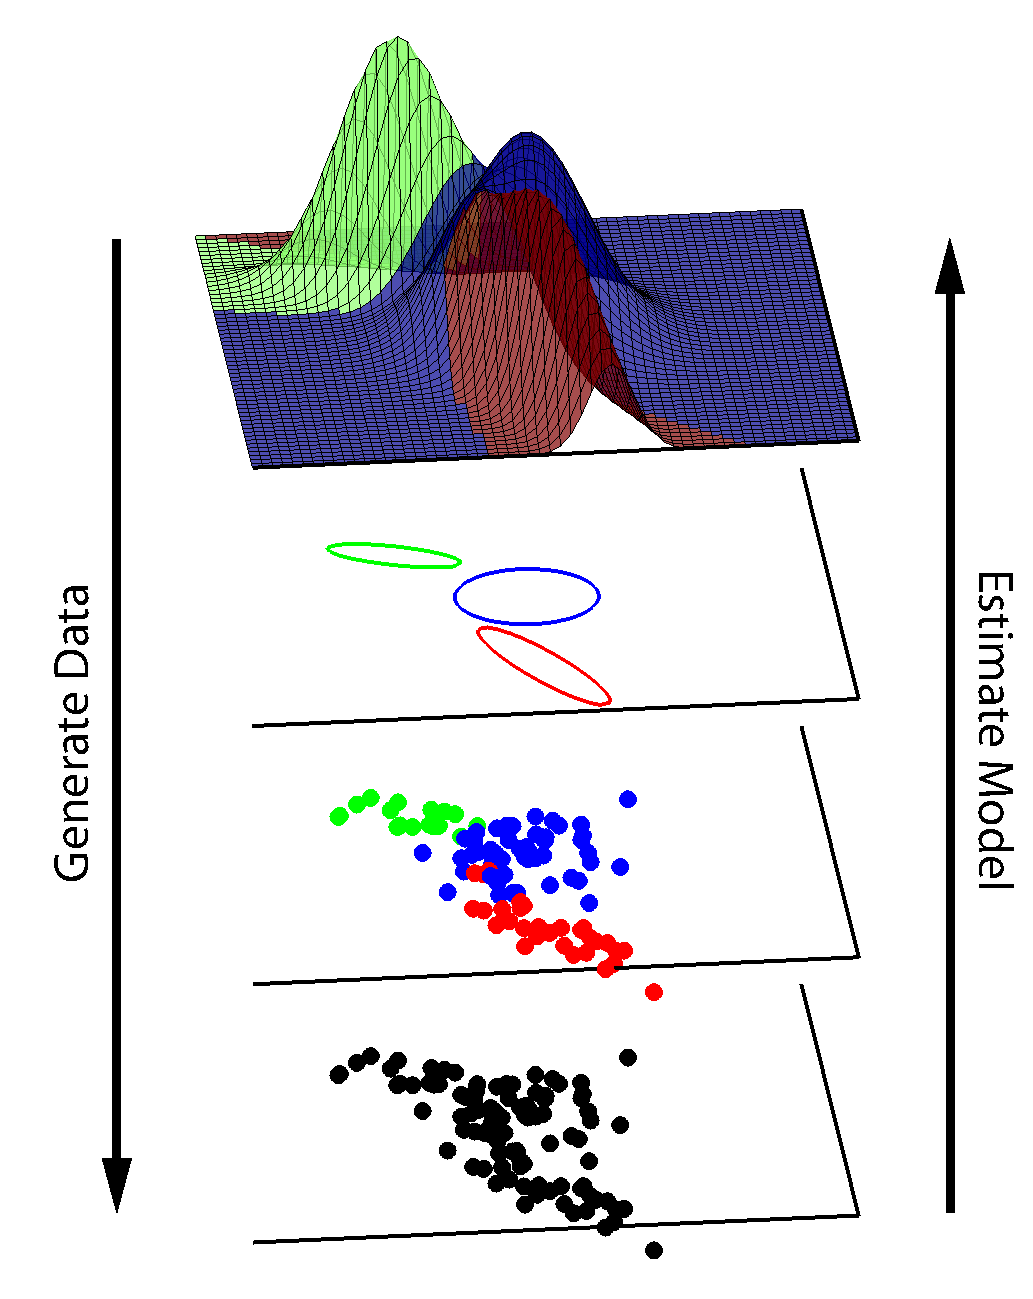
\includegraphics[height=4cm]{generative_model_schematic.pdf}
		%\caption{Generation and estimation.}
%	\end{figure}
\end{center}
\column{.6\textwidth}
\begin{block}{GMM}

\begin{eqnarray*}
\theta_k &=& \{\vec \mu_k,\Sigma_k\} \\
c_i | \vec \pi &\sim& \mbox{Discrete}(\pi_1, \ldots, \pi_K) \\
\vec y_i | c_i=k, \Theta &\sim& \mbox{Gaussian}(\theta_k) \\
\end{eqnarray*}

\end{block}
\end{columns}
%\begin{block}{A challenge to pick the ``best'' model}
%\begin{itemize}
%\item Complexity $\leftrightarrows$ Model selection
%\item Clustering $\leftrightarrows$ Attributing data to clusters
%\end{itemize}
%\end{block}
\begin{block}{Expectation-Maximization}
\[
\begin{array}{llll}
\text{E-step} & T^{(t)}_{i,k} & = & P(c_i = k|\vec{y}_i,\theta^{(t)}_k)\\
& Q(\Theta,\vec{\pi}|\Theta^{(t)},\vec{\pi}^{(t)}) & = & \mathbb{E}[\text{log}L(\Theta,\vec{\pi}|\vec{\mathbf{y}},T^{(t)})] \\
\text{M-step} & (\Theta^{(t+1)},\vec{\pi}^{(t+1)}) & = & \arg\max_{\Theta,\vec{\pi}} Q(\Theta,\vec{\pi}|\Theta^{(t)},\vec{\pi}^{(t)})
\end{array}
\]
\end{block}
\end{frame}

\begin{frame}{}
\begin{columns}[top]
\column{.3\textwidth}
\begin{center}
%		\begin{figure}
		\includegraphics[height=5cm]{gmm_graphical_model.pdf}
		%\caption{Generation and estimation.}
%	\end{figure}
\end{center}
\column{.6\textwidth}
\begin{block}{Bayesian GMM}

\begin{eqnarray*}
\alert{ \Sigma_k} & \alert{\sim} & \alert{\text{IW}_{\nu_0}(\Lambda_0^{-1})}\\
\alert{\vec{\mu}_k} & \alert{\sim} & \alert{\text{Gaussian}(\vec{\mu}_0,\Sigma_k/\kappa_0)} \\
\alert{\vec{\pi}|\alpha} & \alert{\sim} & \alert{\text{Dir}\left(\frac{\alpha}{K},\ldots,\frac{\alpha}{K}\right)} \\
\theta_k &=& \{\vec \mu_k,\Sigma_k\} \\
c_i | \vec \pi &\sim& \mbox{Discrete}(\pi_1, \ldots, \pi_K) \\
\vec y_i | c_i=k, \Theta &\sim& \mbox{Gaussian}(\theta_k) \\
\end{eqnarray*}

\end{block}
\end{columns}
\begin{block}{}
\begin{itemize}
	\item{Inference: sample posterior of $c_i$ via MCMC}
	\item{Applied to spike sorting by \cite{Lewicki1994}.}
\end{itemize}
\end{block}
%\begin{block}{A challenge to pick the ``best'' model}
%\begin{itemize}
%\item Complexity $\leftrightarrows$ Model selection
%\item Clustering $\leftrightarrows$ Attributing data to clusters
%\end{itemize}
%\end{block}
\end{frame}

\begin{frame}
\begin{columns}[top]
\column{.4\textwidth}
\begin{center}
		\begin{figure}
		\includegraphics[height=4cm]{dirichlet_distribution.png}
		%\caption{[source: Wikimedia Commons]}
	\end{figure}
	\tiny{[Source: Wikimedia Commons]}
\end{center}
\column{.5\textwidth}
\begin{block}{Dirichlet Distribution}
\begin{eqnarray*}
\vec{\pi}  & \sim & Dir(\vec{\alpha}) \\
\vec{\alpha} & = & \alpha\vec{H},\,\displaystyle\sum_{i=1}^{K} H_i = 1 \\
\mathbb{E}[\vec{\pi}] & = & \vec{H} \\
\alpha\rightarrow\infty & \Rightarrow & \vec{\pi}\rightarrow\vec{H} \\
\alpha\rightarrow 0 & \Rightarrow & \vec{\pi} \text{ becomes sparse}
\end{eqnarray*}
\end{block}
\end{columns}
\end{frame}

\subsection{Infinite Limit}
\begin{frame}
\begin{eqnarray*}
\vec{\pi} & \sim & \text{Dir}\left(\frac{\alpha}{K},\ldots,\frac{\alpha}{K}\right) \\
P(c_{i+1} = k|c_1,\ldots,c_{i},\alpha) & = & \int P(c_i+1 = k | \vec{\pi}) p(\vec{\pi}|c_1,\ldots,c_{i},\alpha) d\vec{\pi} \\
= \frac{\Gamma(\alpha + i )}{\prod_{j=1}^{K}\Gamma(\frac{\alpha}{K} + n_j)} &&\int\pi_1^{\frac{\alpha}{K}+n_1 -1}\ldots\pi_k^{\frac{\alpha}{K}+n_k}\ldots\pi_K^{\frac{\alpha}{K}+n_K-1}d\vec{\pi} \\
& = & \frac{n_k + \frac{\alpha}{K}}{\alpha + i}
\end{eqnarray*}
Where $n_k$ is the number of $c_j$, $j = 1,\ldots,i$ such that $c_j = k$.   Order the clusters so $n_k > 0$ if $k \le K_+$ and $n_k = 0$ if $k > K_+$.  Then as $K\rightarrow\infty$

\begin{equation*}
P(c_{i+1} = k | c_1,\ldots,c_{i},\alpha) = 
\left\{ \begin{array}{l} 
       \frac{n_k}{\alpha+i} \quad k \leq K_+\\ 
	\frac{\alpha}{\alpha+i} \quad k>K_+ \end{array} \right..
\label{eqn:crp}
\end{equation*}
This is the {\em Chinese Restaurant Process}, $CRP(\alpha)$.
\end{frame}

\begin{frame}
\begin{columns}[top]
\column{.3\textwidth}
\begin{center}
%		\begin{figure}
		\includegraphics[height=7cm]{igmm_graphical_model.pdf}
		%\caption{Generation and estimation.}
%	\end{figure}
\end{center}
\column{.6\textwidth}
\begin{block}{Infinite GMM}

\begin{eqnarray*}
c_i|c_{1:i-1} & \sim & CRP(\alpha)\\
\Sigma_k & \sim & \text{IW}_{\nu_0}(\Lambda_0^{-1})\\
\vec{\mu}_k & \sim & \text{Gaussian}(\vec{\mu}_0,\Sigma_k/\kappa_0) \\
\theta_k &=& \{\vec \mu_k,\Sigma_k\} \\
\vec y_i | c_i=k, \Theta &\sim& \mbox{Gaussian}(\theta_k) \\
\end{eqnarray*}
{\tiny Special case of the Dirichlet Process Mixture Model, due to \cite{Rasmussen2000}}

\end{block}
\end{columns}
\end{frame}

\section{Dirichlet Process}
\subsection{Definition}
\begin{frame}
Dirichlet Process: $\mathcal{G} \sim DP(\alpha,H)$
\begin{itemize}
	\item{$\alpha$ - concentration parameter}
	\item{$H$ - base distribution}
	%\item{Given a finite partition $\{\Theta_1,\ldots,\Theta_K\}$, $(\mathcal{G}(\Theta_1),\ldots,\mathcal{G}(\Theta_K)) \sim Dir(\alpha H(\Theta_1),\ldots,\alpha H(\Theta_K))$}
	\item{$\mathcal{G}$ is {\em atomic:} $p(\theta|\mathcal{G}) = \displaystyle\sum_{k=1}^{\infty} \pi_k \delta(\theta-\theta_k)$}
\end{itemize}
\begin{figure}
\includegraphics[scale=0.5]{dp_draw.pdf}
\begin{columns}[bottom]
\column{.5\textwidth}
\begin{center}
$H =$ Gaussian$(0,1)$
\end{center}
\column{.5\textwidth}
\begin{center}
$\mathcal{G} \sim DP(100,H)$
\end{center}
\end{columns}
\end{figure}
\end{frame}

\subsection{Stick Breaking Construction}
\begin{frame}
\begin{eqnarray*}
\pi'_k & \sim & Beta(1,\alpha) \\
\pi_k & = & \pi'_k \prod_{i=1}^{k-1}(1-\pi_i) \\
\theta_k & \sim & H \\
\mathcal{G} & = & \sum_{k=1}^{\infty} \pi_k \delta_{\theta_k}
\end{eqnarray*}
\end{frame}

\subsection{P\'{o}lya Urn Scheme and CRP}
\begin{frame}
Draws $x_{1:i} \sim \mathcal{G}$ cluster together.  Let $K_+$ be the number of distinct values of $x_{1:i}$, $n_k$ be the number of draws with value $\theta_k$. 
\begin{equation*}
\mathcal{G}|x_{1:i} \sim DP\left(\alpha + i, \sum_{k=1}^{K_+} \frac{n_k}{\alpha + i}\delta_{\theta_k} + \frac{\alpha}{\alpha+i}H\right)
\end{equation*}
\begin{equation*}
x_{i+1}|x_{1:i} \sim \sum_{k=1}^{K_+} \frac{n_k}{\alpha + i}\delta_{\theta_k} + \frac{\alpha}{\alpha+i}H
\end{equation*}
\end{frame}

\subsection{Extensions}
\begin{frame}
\begin{block}{Pitman-Yor Process}
$\mathcal{G} \sim PY(\alpha,d,H)$,  $PY(\alpha,0,H) \Leftrightarrow DP(\alpha,H)$
\begin{itemize}
\item{$d \in [0,1]$:  discount}
\item{Stick breaking construction: $\pi'_k \sim$ Beta$(1-d,c+kd)$}
\item{CRP construction:}
\begin{equation*}
P(c_{i+1} = k | c_1,\ldots,c_{i},\alpha,d) = 
\left\{ \begin{array}{l} 
       \frac{n_k - d}{\alpha+i} \quad k \leq K_+\bigskip\\ 
	\frac{\alpha + kd}{\alpha+i} \quad k>K_+ \end{array} \right..
\label{eqn:pyp-crp}
\end{equation*}

\end{itemize}
\end{block}
\end{frame}

\begin{frame}
\begin{columns}[top]
\column{.5\textwidth}
\begin{center}
		\begin{figure}
		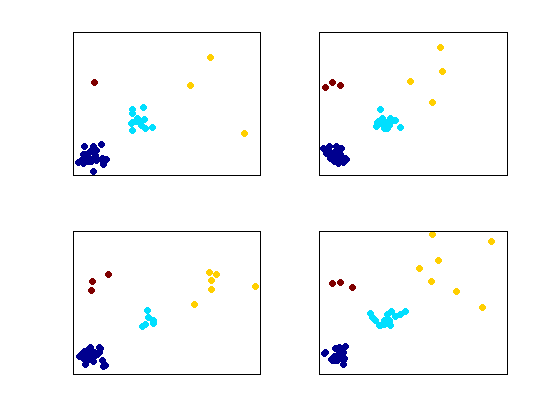
\includegraphics[height=4cm]{shared_clustering.png}
		%\caption{[source: Wikimedia Commons]}
	\end{figure}
\end{center}
\column{.5\textwidth}
\begin{block}{Hierarchical Dirichlet Process}
Share clusters across groups of data
\begin{eqnarray*}
\mathcal{G}_0  & \sim & DP(\alpha,H) \\
\mathcal{G}_j & \sim & DP(\alpha,\mathcal{G}_0) \\
\theta_{ji} & \sim & \mathcal{G}_j
\end{eqnarray*}
\end{block}
\end{columns}
\begin{block}{Applications}
\begin{itemize}
\item{Infinite HMM - each $\mathcal{G}_j$ is the transition probability given a state \citep{Teh2006b}.}
\item{Variable-length Markov models for language data \citep{Teh2006a}.}
\end{itemize}
\end{block}
\end{frame}

\section{Conclusion}

\subsection{My Research}
\begin{frame}
\begin{itemize}
\item{Discrete time, discrete alphabet sequence learning}
\item{Learn probabilistic deterministic finite automata}
\begin{itemize}
	\item{Subclass of HMMs}
	\item{Intermediate between variable-length Markov models and full HMM}
	\item{Use HDP as prior for transition matrix, similar to infinite HMM}
	\item{Inference via Metropolis-Hastings}
	\item{Works on small regular grammars ($\sim$7 states), currently extending to richer data}
\end{itemize}
\end{itemize}
\end{frame}

\subsection{Recap}
\begin{frame}
Nonparametric Bayesian models sidestep the model selection problem, combining model estimation and model selection into one.  We define the Dirichlet Process and use it as a prior over parameters that controls the clustering of data.  We show that the DP emerges in the limit of certain parametric models as the number of parameters goes to infinity.  Draws from a DP can be marginalized out, yielding a tractable model that can be estimated by standard Bayesian methods.  The DP can be extended in various ways, and we are applying these tools to discrete alphabet sequence learning with as few free parameters as possible.
\end{frame}

\subsection{Credit}
\begin{frame}
Many thanks to:
\begin{itemize}
	\item{Frank Wood}
	\item{Liam Paninski}
	\item{Nick Bartlett}
\end{itemize}
With support provided by NSF GRFP.\bigskip\\

References:
\bibliographystyle{plainnat}
\bibliography{../../papers/uber} 
\end{frame}

\end{document}